\ylDisplay{Lääts} % Ülesande nimi
{Mihkel Kree} % Autor
{lahtine} % Voor
{2015} % Aasta
{G 5} % Ülesande nr.
{5} % Raskustase
{
% Teema: Geomeetriline-optika
\ifStatement
Joonisel on kujutatud objekt AB ning sellest kumerläätses tekkinud tõeline kujutis A'B'. Leidke konstrueerimise teel läätse keskpunkti ning fookuse asukoht.

\begin{center}
 \includegraphics[width=0.7\linewidth]{2015-lahg-05-laatsMihkel.pdf}
\end{center}
\fi


\ifHint
Läätse asukoha leidmiseks tasub vaadata geomeetriliselt omapäraseid kiiri ja kuidas need läbi läätse murduvad. Selleks sobivad näiteks kiired AB, AA' ja BB'.
\fi


\ifSolution
Paneme esmalt tähele, et läätse keskpunkti läbivad kiired AA' ja BB' ei murdu. Seega paikneb läätse keskpunkt O lõikude AA' ja BB' lõikepunktis. Teisalt märkame, et valguskiir AB murdub valguskiireks A'B'. Niisiis, pikendades lõike AB ja A'B', leiame nende lõikepunkti X. Sellega oleme konstrueerinud läätse tasandi OX. Läätse optilise peatelje leiame, kui tõmbame läätse tasandiga ristuva sirge s läbi läätse keskpunkti O. Fookuse F leidmiseks konstrueerime näiteks peateljega paralleelse kiire AC, mis murdub läbi fookuse.

\begin{center}
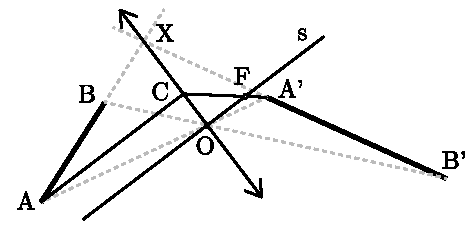
\includegraphics[width=\textwidth]{2015-lahg-05-laatsLahendus.pdf}
\end{center}
\fi


\ifEngStatement
% Problem name: Lens
The figure shows an object AB and its real image A’B’ made by a convex lens. Find the locations of the lens’ center and the focal point, by construction.
\begin{center}
 \includegraphics[width=0.7\linewidth]{2015-lahg-05-laatsMihkel}
\end{center}
\fi


\ifEngHint
To find the location of the lens you should observe geometrically unique rays and how they refract through the lens. For example the rays AB, AA’ and BB’ are suitable for that.
\fi


\ifEngSolution
Let us first notice that the rays AA’ and BB’ going through the center of the lens do not refract. Therefore the center of the lens O is located in the intersection of the sections AA’ and BB’. Let us also notice that the ray AB is refracted into the ray A’B’. So, extending the sections AB and A’B’ we find their intersection X. With this we have constructed the plane of the lens OX. We find the optical axis of the lens if we draw a line s perpendicular to the plane of the lens through the center of the lens O. To find the focal point F we can construct a ray AC parallel to the main axis that refracts through the focal point. 
\begin{center}
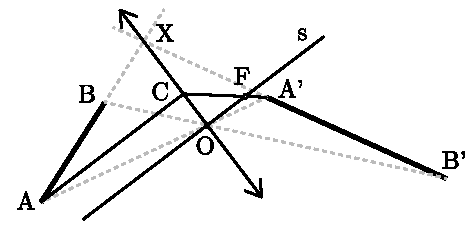
\includegraphics[width=\textwidth]{2015-lahg-05-laatsLahendus}
\end{center}
\fi
}